\documentclass[12pt]{article}
\usepackage{amssymb}
\usepackage{amsmath}
\usepackage{tikz}
\usetikzlibrary{arrows, positioning}
\begin{document}
    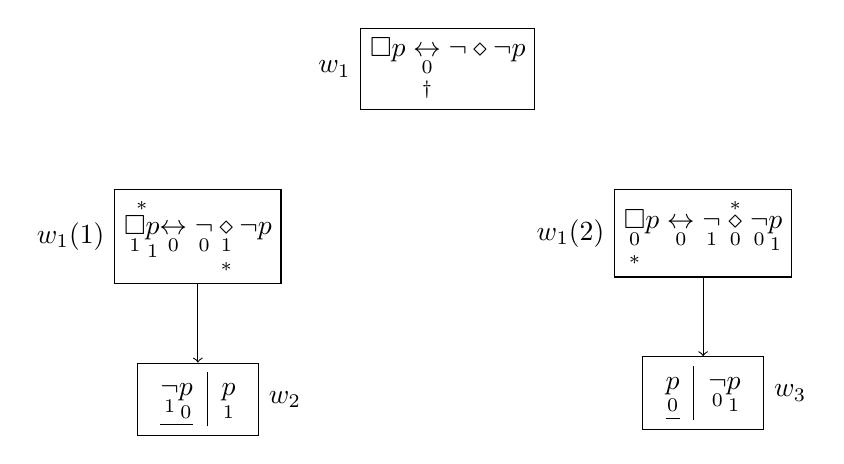
\begin{tikzpicture}[
    world/.style={rectangle,draw},
    invisible/.style={rectangle}]
        \node[world] (w_1)
            { $\Box p \underset{\dagger}{\underset{0}{\leftrightarrow}} \neg \diamond \neg p$
            };

        \node[black, left] at (w_1.west) {$w_1$};

        \node[world] (w_1') [below left=of w_1]
            { $\stackrel{*}{\underset{1}{\Box} \underset{1}{p}} \underset{0}{\leftrightarrow} \underset{0}{\neg} \underset{*}{\underset{1}{\diamond}} \neg p$
            };

        \node[black, left] at (w_1'.west) {$w_1(1)$};

        \node[world] (w_2) [below=of w_1']
            { $\begin{array}{c|c}
                \underline{\underset{1}{\neg}\underset{0}{p}} &
                \underset{1}{p}
            \end{array}$
            };

        \node[black, right] at (w_2.east) {$w_2$};

        \node[world] (w_1'') [below right=of w_1]
            { $\underset{*}{\underset{0}{\Box}} p \underset{0}{\leftrightarrow} \underset{1}{\neg} \stackrel{*}{\underset{0}{\diamond}} \underset{0}{\neg} \underset{1}{p}$
            };

        \node[black, left] at (w_1''.west) {$w_1(2)$};

        \node[world] (w_3) [below=of w_1'']
            { $\begin{array}{c|c}
                \underline{\underset{0}{p}} &
                \underset{0}{\neg}\underset{1}{p}
            \end{array}$
            };

        \node[black, right] at (w_3.east) {$w_3$};

        \draw[->] (w_1') -- (w_2);
        \draw[->] (w_1'') -- (w_3);

    \end{tikzpicture}
\end{document}
